\documentclass[11pt]{article}
\usepackage[margin=1in]{geometry}
\usepackage{amsmath,amssymb,amsthm,bm}
\usepackage{hyperref}
\usepackage{graphicx}
\usepackage{caption}
\usepackage{listings}
\usepackage{xcolor}
\usepackage{float}
\usepackage{placeins}

% Graphics path
\graphicspath{{figures/}}

% Listings style for code
\lstdefinestyle{code}{%
  language=Python,
  basicstyle=\ttfamily\small,
  numbers=left,
  numberstyle=\tiny,
  keywordstyle=\color{blue}\bfseries,
  commentstyle=\color{teal!70!black},
  stringstyle=\color{orange!70!black},
  breaklines=true,
  frame=single,
  rulecolor=\color{black!30},
  tabsize=2,
  showstringspaces=false
}
\lstset{style=code}

\title{Support Vector Machines: Theory and Practice}
\author{}
\date{\today}

\begin{document}
\maketitle

\section{Introduction}
Support Vector Machines (SVMs) are margin-based learners that find a decision boundary maximizing the margin between classes. With kernels, they represent complex non-linear decision boundaries while remaining convex to optimize.

\section{Theory and Formulas}
For linear, soft-margin SVM in primal form, given labeled data $\{(\mathbf{x}_i, y_i)\}_{i=1}^n$ with $y_i\in\{-1,+1\}$:
\begin{align}
\min_{\mathbf{w}, b, \boldsymbol{\xi} \ge 0} \quad & \tfrac{1}{2}\lVert \mathbf{w} \rVert^2 + C \sum_{i=1}^n \xi_i \\
\text{s.t.} \quad & y_i (\mathbf{w}^\top \mathbf{x}_i + b) \ge 1 - \xi_i, \; i=1,\dots,n.
\end{align}
In the dual, data appear only via inner products; replacing them with kernels $K(\mathbf{x},\mathbf{x}')$ provides non-linear SVMs. The decision function is
\begin{equation}
f(\mathbf{x}) = \sum_{i \in SV} \alpha_i y_i K(\mathbf{x}_i, \mathbf{x}) + b, \quad \hat{y} = \mathrm{sign}\, f(\mathbf{x}),
\end{equation}
where $SV$ are support vectors with non-zero multipliers $\alpha_i$. RBF kernel $K(\mathbf{x},\mathbf{x}') = \exp(-\gamma \lVert \mathbf{x}-\mathbf{x}'\rVert^2)$ is a common default. Hyperparameters $C$ (slack penalty) and $\gamma$ (kernel width) control regularization and boundary complexity.

\section{Applications and Tips}
\begin{itemize}
  \item \textbf{Scaling:} always scale features; SVMs are sensitive to feature scales.
  \item \textbf{Hyperparameters:} tune $C$ and $\gamma$ (for RBF) via cross-validation; start with $C\in[0.1,10]$, $\gamma\in[10^{-2},10]$ (log grid).
  \item \textbf{Class imbalance:} use \texttt{class\_weight=balanced} to reweight classes.
  \item \textbf{Probability:} \texttt{SVC} supports probability with \texttt{probability=True} (adds calibration cost); otherwise use \texttt{decision\_function}.
  \item \textbf{Multiclass:} \texttt{SVC} uses one-vs-one internally; \texttt{LinearSVC} uses one-vs-rest.
\end{itemize}

\section{Python Practice}
Run the script in this chapter directory to generate figures into \texttt{figures/}.
\begin{lstlisting}[style=code,caption={Generate SVM figures},label={lst:genfigs_svm}]
python gen_svm_figures.py
\end{lstlisting}

% Include the full Python source
\lstinputlisting[style=code,caption={gen\_svm\_figures.py},label={lst:source_svm}]{gen_svm_figures.py}

\section{Result}
\begin{figure}[H]
  \centering
  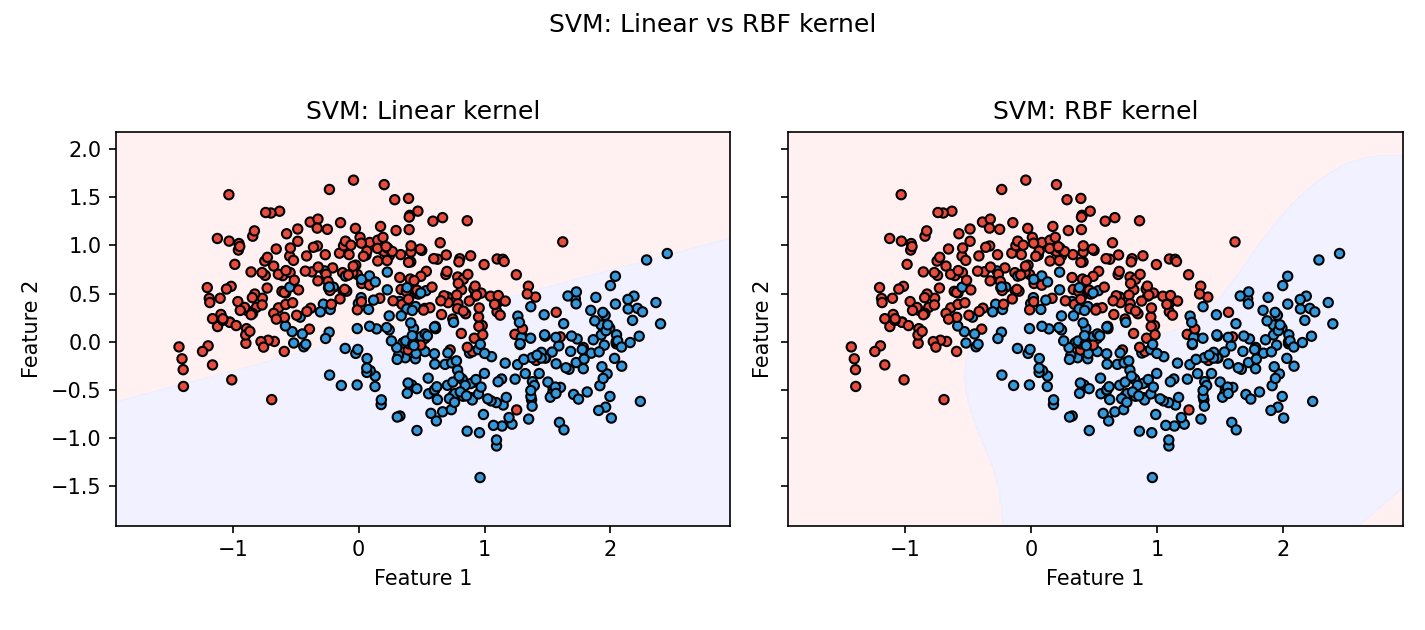
\includegraphics[width=0.95\linewidth]{svm_linear_vs_rbf.png}
  \caption{SVM decision boundaries: linear vs RBF kernel.}
  \label{fig:svm_lin_rbf}
\end{figure}
\FloatBarrier

\begin{figure}[H]
  \centering
  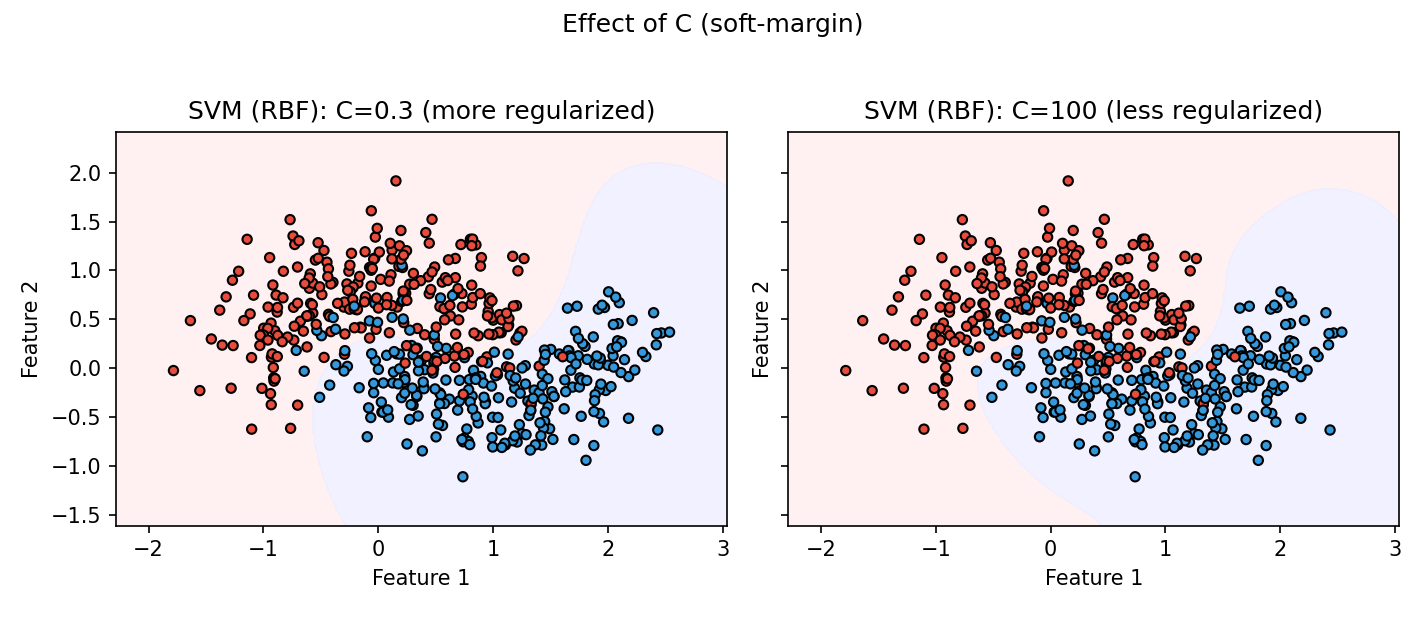
\includegraphics[width=0.95\linewidth]{svm_C_compare.png}
  \caption{Effect of soft-margin parameter C (RBF kernel).}
  \label{fig:svm_c}
\end{figure}
\FloatBarrier

\begin{figure}[H]
  \centering
  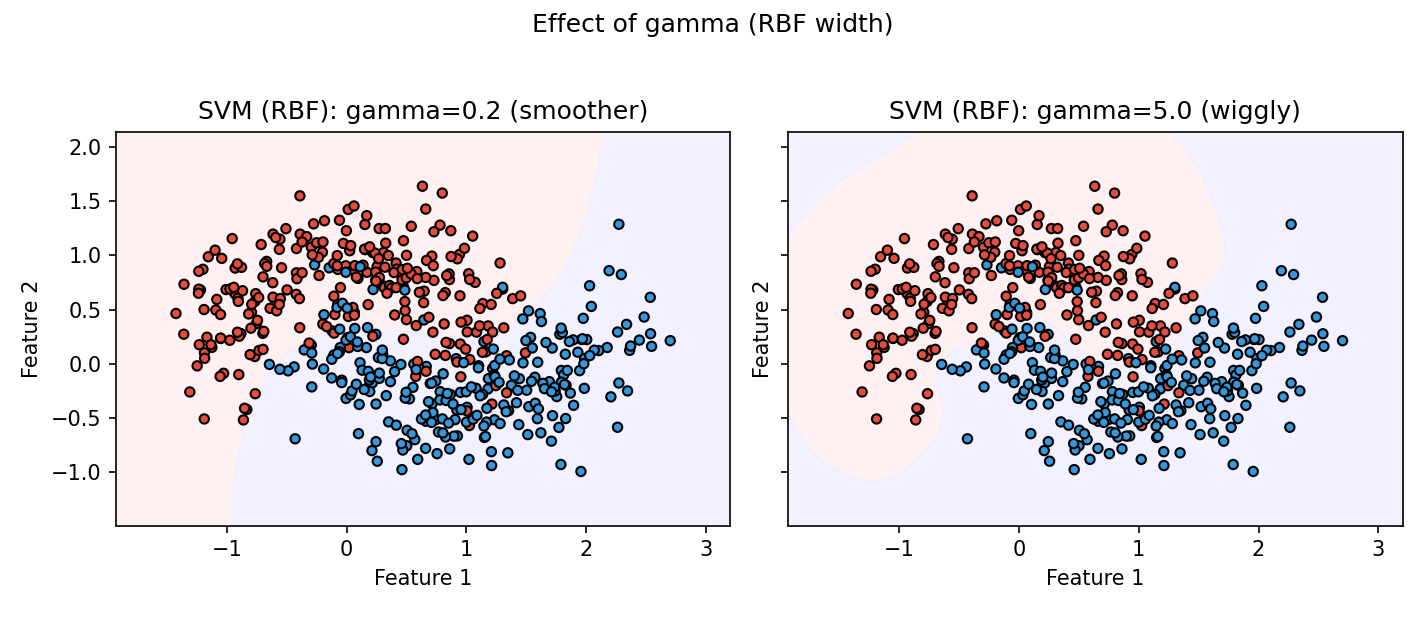
\includegraphics[width=0.95\linewidth]{svm_gamma_compare.png}
  \caption{Effect of RBF gamma on boundary smoothness.}
  \label{fig:svm_gamma}
\end{figure}
\FloatBarrier

\begin{figure}[H]
  \centering
  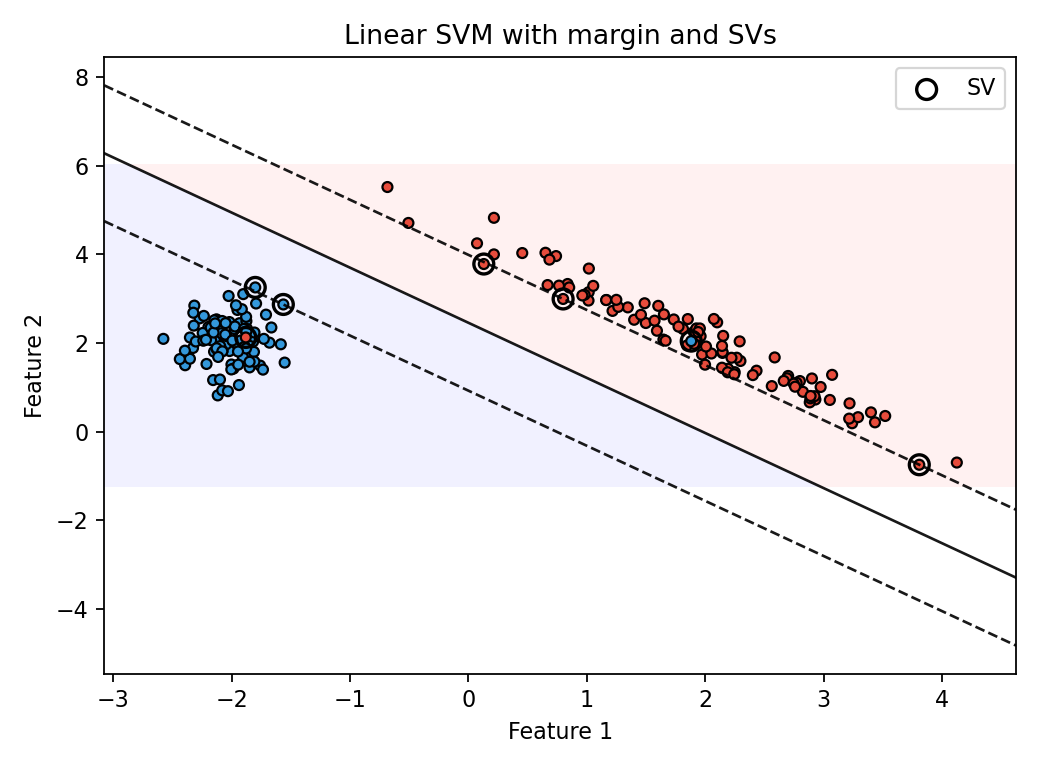
\includegraphics[width=0.85\linewidth]{svm_margin_support_vectors.png}
  \caption{Linear SVM: margin lines and highlighted support vectors.}
  \label{fig:svm_margin}
\end{figure}
\FloatBarrier

\begin{figure}[H]
  \centering
  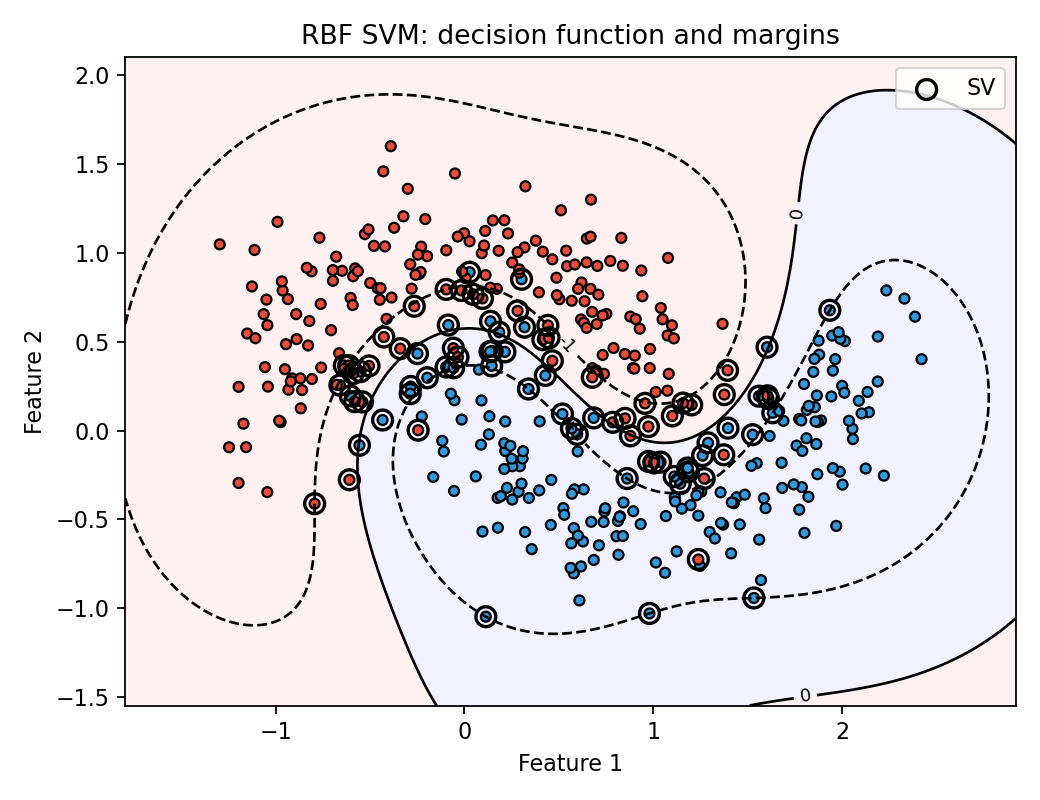
\includegraphics[width=0.85\linewidth]{svm_decision_function.png}
  \caption{RBF SVM decision function: contours at -1, 0, +1.}
  \label{fig:svm_df}
\end{figure}
\FloatBarrier

\section{Summary}
SVMs maximize margins for robust classification and extend to non-linear problems via kernels. With proper scaling and tuning of $C$ and kernel parameters, they deliver strong performance across many domains.

\end{document}

